\documentclass[devoir3.tex]{subfiles}

\begin{document}

\section*{Question 2}
Donnez toutes les étapes de l’algorithme de Floyd pour calculer le plus court chemin entre toutes les paires de noeuds du graphe de la figure \ref{fig:fig1}. Donnez la matrice obtenue à chaque itération.

\begin{figure}[H]
	\centering
	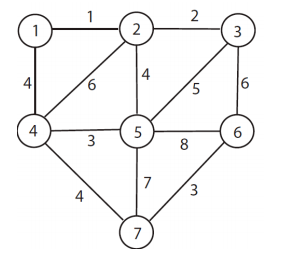
\includegraphics[width=8cm]{fig1}
	\caption{Graphe}
	\label{fig:fig1}   
\end{figure}

\end{document}
